\documentclass[a4paper]{article}

\usepackage[english]{babel}
\usepackage[utf8]{inputenc}

\usepackage{amsmath}
\usepackage{amssymb}
\usepackage{enumerate}
\usepackage{hyperref}
\usepackage{graphicx}
\usepackage{subcaption}

\usepackage{natbib}
\bibliographystyle{plainnat}
\bibpunct{(}{)}{;}{a}{,}{,}

\usepackage{mythm}

\DeclareMathOperator*{\argmax}{arg\,max} % argmax operator
\def\regret{R}
\def\regretHAT{\hat{R}}


%%%%%%%%%%%%%%%%%%%%%%%%%%%%%%%%%%%%%%%%%%%%%%%%%%%%%%%%%%%%%%%
\begin{document}
%%%%%%%%%%%%%%%%%%%%%%%%%%%%%%%%%%%%%%%%%%%%%%%%%%%%%%%%%%%%%%%

\title{Active Multi-Armed Bandits}
\author{Jan Leike et al.}
% + Owain Evans + David Kruger + John Salvatier
\date{\today}

\maketitle


\begin{abstract}%
We introduce the \emph{active multi-armed bandit problem},
a cross-over between multi-armed bandits and active learning.
%~\citep{Settles:2010}.
% Despite being a slight variation on the simplest reinforcement learning problem,
% active multi-armed bandits turn out to be quite challenging:
As a sub-problem of the hard class of partial monitoring problems,
the problem incurs $\Theta(n^{2/3})$ worst-case regret.
Moreover,
the quality of an arm is not independent of the other arms
and greedy information-gathering strategies perform poorly.
% Therefore good strategies need to think globally about the problem.
We compare partial monitoring algorithms on the problem and
introduce a new algorithm that outperforms them.
However,
the central question to solving active multi-armed bandits,
how to efficiently quantify the long-term value of information,
remains open.
\end{abstract}



%%%%%%%%%%%%%%%%%%%%%%%%%%%%%%%%%%%%%%%%%%%%%%%%%%%%%%%%%%%%%%%
\section{Problem Formulation}
%%%%%%%%%%%%%%%%%%%%%%%%%%%%%%%%%%%%%%%%%%%%%%%%%%%%%%%%%%%%%%%

%\paragraph{Setup.}
The \emph{active multi-armed bandit problem} is
an online learning problem
where the learner has to select from $K$ actions (`arms') in every round.
Choosing action $I_t \in \{ 1, \ldots, K \}$ in round $t$
incurs a payoff $X_t$ of
drawn from a time-independent distribution $\nu_{I_t}$
with mean $\mu_i$ unknown to the learner.
In contrast to the classical multi-armed bandit problem,
the learner does not observe the payoff
unless they pay a fixed \emph{query cost $c > 0$}.
This cost is the same for every arm and every round.

%\paragraph{Objective.}
Let $\mu^* := \max_i \mu_i$ denote the mean of the best arm.
The goal of the learner is to maximize expected payoff up to a known horizon $n$,
or, equivalently, to minimize the \emph{expected regret}
\[
\regret_n = \mathbb{E} \left[ \sum_{t=1}^n (\mu^* - X_t - c Q_t) \right],
\]
where $Q_t$ is $1$ if the learner chooses to observe the reward in round $t$ and $0$ otherwise.
In other words, the expected regret is the expected payoff
that is lost
because the learner did not blindly choose the best option in every round.
% (note that $Q_t$ is a random variable).

% \paragraph{Notation.}
% Let $i^* := \argmax_i \mu_i$ be an index of an optimal arm,
% let $\Delta_i := \mu^* - \mu_i$, and
% let $\Delta_{\min} := \min_{i \neq i^*} \Delta_i$.



%%%%%%%%%%%%%%%%%%%%%%%%%%%%%%%%%%%%%%%%%%%%%%%%%%%%%%%%%%%%%%%
\section{Properties}
%%%%%%%%%%%%%%%%%%%%%%%%%%%%%%%%%%%%%%%%%%%%%%%%%%%%%%%%%%%%%%%

%\paragraph{Partial monitoring.}
The active multi-armed bandit problem is
a subproblem of the partial monitoring problem~\citep{Piccolboni01}:
the action space consists of the $2K$ actions (the $K$ arms with and without querying) and
the feedback is the observed payoff or a blank symbol.
In contrast to most of the literature on partial monitoring,
we consider the environment to be stochastic instead of adversarial.
For distributions with finitely many payoffs (such as Bernoulli distributions),
active multi-armed bandits are
stochastic finite partial monitoring problems~\citep{Komiyama15}.
In case of two outcomes,
(adversarial) partial monitoring problems can be classified in four different
categories: $0$, $\Theta(n^{1/2})$, $\Theta(n^{2/3})$, or $\Theta(n)$ regret~\citep{Antos13}.
These categories are called trivial, easy, hard, and hopeless respectively.
While multi-armed bandits fall into the easy category,
\emph{active} multi-armed bandits fall into the hard category:

% TODO: partial monitoring with graph feedback, see "Online learning with feedback graphs: beyond bandits." COLT 2015.

\begin{proposition}[Cost-Independent Regret Bound]
The worse-case expected regret is
\[
\inf_\pi \sup_{\mu_1, \ldots, \mu_K} \regret_n \in \Theta(n^{2/3}).
\]
% and the problem-dependent regret bound is $\regret_n \in \Theta(\sum_{i: \Delta_i > 0} \log(n)/\Delta_i)$.
\end{proposition}
\begin{proof}[Proof sketch.]
Consider an active two-armed bandit problem
where the gap between the arms is $\Delta := n^{-1/3}$.
Commiting blindly to one of the arms incurs a regret of
$0.5n \cdot n^{-1/3} \in \Theta(n^{2/3})$.
Alternatively, to distinguish the arms,
we need $\Theta(1/\Delta^2)$ steps.
In every step we need to pay the cost $c$ to see the payoff,
which incurs a regret of
at least $c\Theta(1/\Delta^2) = \Theta(cn^{2/3})$.
% This also leads to the problem-dependent regret bound of $\Theta(1/\Delta_{\min}^2)$.
\end{proof}

%\paragraph{Active bandits vs.\ regular bandits.}
Intuitively, the fundamental difference to (regular) multi-armed bandit problems is in the cost of distinguishing two very close arms.
In active bandits, distinguishing two close arms incurs regret linear in the number of time steps needed to distinguish them ($n^{2/3}$ in the worst case), whereas in (regular) bandits the regret grows proportionally to the gap size ($n^{1/2}$ in the worst case).

%\paragraph{Cost-dependent regret.}
To achieve optimal asymptotic regret, we can ignore the magnitude of the query cost, since it is constant.
Partial monitoring algorithms are designed for optimal asymptotic regret rate and do not take the magnitude of the query cost into account.
Here we are particularly interested in optimizing
the cost-dependent regret.

%\paragraph{Query and then stop.}
The optimal strategy is to query for a number of time steps
and then stop querying altogether.
If you don't query, then in the next step you face the same information,
except that the horizon is now shorter,
so the value of information can only have diminished.

%\paragraph{Regular bandits as edge cases.}
Active multi-armed bandit problems degenerate into two familiar problems in the edge cases.
If $c = 0$ we face a regular bandit problem and the regret $\regret_n$ corresponds to the cumulative regret.
If $c \gg X_t$,
then $\regret_n$ is dominated by the simple regret
(the gap of the chosen arm) and
we have a best arm identification problem.
But there is a trade-off between
simple regret and cumulative regret~\citep[Thm.~1]{Bubeck11}:
if the cumulative regret is small,
then there is a lower bound on the simple regret.
Any algorithm for a moderate cost setting therefore
has to manage the balancing act between cumulative and simple regret.


%%%%%%%%%%%%%%%%%%%%%%%%%%%%%%%%%%%%%%%%%%%%%%%%%%%%%%%%%%%%%%%
\section{Algorithms}
%%%%%%%%%%%%%%%%%%%%%%%%%%%%%%%%%%%%%%%%%%%%%%%%%%%%%%%%%%%%%%%

%\paragraph{Our goal.}
For finite sets of payoffs,
PM-DMED achieves the optimal cost-independent regret rate~\citep{Komiyama15}.
We are looking for a (heuristic) algorithm that achieves optimal asymptotic (cost-dependent) regret rate,
performs well in practice and has constant or linear time complexity.
Ideally, the algorithm's performance does not degrade at the edge cases with $c = 0$ and $c \gg \max_i \Delta_i$.

%\paragraph{Bayes-optimal solution for Bernoullis.}
If $\nu_1, \ldots \nu_K$ are Bernoulli distributions,
then the Bayes-optimal solution
can be found with dynamic programming:
The corresponding belief MDP has $\mathcal{O}(n^{2K})$ states
and can be solved in $\mathcal{O}(n^{2K})$ time steps.
This is polynomial for constant $K$,
but completely prohibitive in practice.

%\paragraph{Optimism cannot work.}
It is well-known that to solve partial monitoring problems
it is sometimes necessary to take actions that you strongly believe to be suboptimal to get information.
For active bandits, paying to see the reward is always suboptimal
by at least $c > 0$.
Nevertheless, if we never pay the cost, we learn nothing about the problem.
Because of this, strategies like optimism or Thompson sampling cannot work here.

%\paragraph{No index strategy.}
Moreover, there can be no index strategy~\citep[Ex.~4]{Hay12}.
An index strategy computes for each arm
a number that is independent of the other arms
and takes the action with highest number.
% This requires that
% the the quality of an action is independent of the alternatives.
Consider the following 3-armed active bandit problem
where the decision between arm 1 and arm 2 depends
on the value of arm 3:
The arms' payoffs are deterministic but unknown with
either $-1.5$ or $1.5$ for arm 1 with equal probability,
either $0.25$ or $1.75$ for arm 2 with equal probability, and
$\lambda$ for arm 3.
The horizon is $n = 1000$
and the query cost is $c = 200$.
% for $\lambda = 1.31$ observing arm 1 is not worth the investment, but observing arm 2 is worth $n (1.75 - \lambda) \cdot 0.5 - 200 = 40 > 0$.
% For $\lambda = -10$, observing arm 1 and then blindly switching to arm 2 if the payoff is $-1.5$ yields expected value of $((n-1)1 - 1.5) \cdot 0.5 + n 1.5 \cdot 0.5) - 200 = 1047.5$.
% Blindly commiting to the second arm has an expected value of $1000$. Observing the second arm and then observing the first arm if the second arm is $0.25$ has an expected value of
% $(n1.75 - 200) \cdot 0.5 + (0.25 + (n-1)1.5 - 400) \cdot 0.25 + (-1.5 + (n-1)0.25 - 400) \cdot 0.25 = 1011.75$.
% Hence observing arm 2 is optimal for $\lambda = 1.31$ and observing arm 1 is optimal for $\lambda = -10$.
% In short:
If $\lambda$ is high (e.g.\ $1.31$),
we want to observe the arm with the high maximum first
since the other arm is known to be suboptimal, and
if $\lambda$ is low (e.g.\ $-10$),
we want to observe the arm with high variance first
because in case that arm is bad, we are sure that
the high mean arm is better and don't need to observe it.

%then observing mu_1 is -0.2 in expectation, but in case the observation is -1.5, it's worth switching to arm 2 and we get an expectation of 1 - 0.2 = 0.8. If the payoff is 1.5, then it's not worth observing/switching to arm 2. So we get 0.8 * 0.5 + 1.3 * 0.5 = 1.05. Blindly commiting to arm 2 is 1. Observing mu_2 = 0.25 leads us to query mu_1 to get 1.5*0.5 + 0.25*0.5 - 2*0.2 = 0.475. Hence pull second first has 1.55*0.5 + 0.475*0.5 = 1.0125.
% Need n = 1000 and rescale rewards by 0.001 so that the query steps don't matter.
% In short: if lambda is high, observe the high max arm, and if lambda is low, observe the high variance arm first (because if it's bad, you don't need to observe the other one, just commit to it).

%\paragraph{Knowledge gradients}
If $\nu_1, \ldots \nu_K$ are Gaussian distributions,
then we can estimate the value of paying the query cost for multiple time steps using
a knowledge gradient~\citep[Ch.~5]{PowellRyzhov12}.
As far as we know, how to efficiently compute the multi-step knowledge gradient for Bernoulli bandits is still an open question.

% KG is optimal when N = 1. We will show that KG
% is optimal in two other special cases: first, when there are only two alternatives to
% measure; second, when the measurements are free from noise, (σ ε ) 2 = 0, and when
% the parameters of the time 0 prior can be ordered by μ 01 ≥ μ 02 ≥ . . . ≥ μ 0 M and
% 0 ≥ σ 0 ≥ . . . ≥ σ 0
% σ 11
% 22
% M M

% Wang et al.: The Knowledge Gradient for Sequential Decision Making with Stochastic Binary Feedbacks. Does knowledge gradient for sorta-linear bandits but with binary feedback

%\paragraph{Bernoulli has no greedy solution.}
In Bernoulli bandits, this problem does not have a greedy solution:
Usually one additional data point does not change our opinion
which arm we currently consider to be best.
So a greedy strategy considers the value of information to be zero and stops querying prematurely.
Therefore we have to take into account the long-range effects of querying for multiple time steps.
As far as we know, how to efficiently compute the knowledge gradient in this setting is still an open question.
% TODO: tricky because the posterior is nonstationary.



%%%%%%%%%%%%%%%%%%%%%%%%%%%%%%%%%%%%%%%%%%%%%%%%%%%%%%%%%%%%%%%
\section{Experiments}
%%%%%%%%%%%%%%%%%%%%%%%%%%%%%%%%%%%%%%%%%%%%%%%%%%%%%%%%%%%%%%%

Our algorithms:
\begin{itemize}
\item DMED~\citep{Honda10} with commitment when 1 arm is selected
\item PM-DMED~\citep{Komiyama15}
\item optimal fixed query stopping time (optimized problem-dependent)
\item mind-changing-cost heuristic (optimized $\alpha$ problem-dependent)
\item knowledge gradient
\end{itemize}

Neither MCCH nor the knowledge gradient are index strategies.

\iffalse
Problems:
* medium query cost c = 2 (>> gap)
  * horizon n = 10k vs gap 0.1 (< n^2/3)
  * horizon n = 1k vs gap 0.1 (~ n^2/3)
  * horizon n = 10k vs gap 0.01 (don't identify the arms)
* high query cost c = 50
  * horizon n = 10k vs gap 0.3 (pay to identify)
  * horizon n = 10k vs gap 0.1 (borderline case)
  * horizon n = 10k vs gap 0.05 (do not pay to identify)
* low query cost c = 0.01 (c << gap)
  * horizon n = 10k vs gap 0.1 (should almost always find the best arm)
  * horizon n = 200 vs gap 0.1 (query all the way?)

Also: plot regret vs different query stopping times and different alpha
\fi


%%%%%%%%%%%%%%%%%%%%%%%%%%%%%%%%%%%%%%%%%%%%%%%%%%%%%%%%%%%%%%%
\subsection{Mind-Changing Cost Heuristic}
%%%%%%%%%%%%%%%%%%%%%%%%%%%%%%%%%%%%%%%%%%%%%%%%%%%%%%%%%%%%%%%

We introduce a new algorithm called \emph{mind-changing cost heuristic}~(\texttt{MCCH}).
Let $\hat{m}$ be an estimate of the expected number of time steps
we need to query in succession to move the posterior mean of the second best arm to the posterior mean of the best arm
(we use $\hat{m} := \max\{ 1, \lceil 2\min_i ((T_i + 1) \hat{\Delta}_i)^2 \rceil \}$).
Let $\regretHAT_n(i)$ denote the Bayes-expected regret
when committing to arm $i$ now (never querying again) and
let $\hat{i}$ denote the current estimate of the best arm.
%
The algorithm pays the query cost if and only if
\begin{equation}\label{eq:PRQ-criterion}
c\hat{m} < \alpha \regretHAT_n(\hat{i})
\end{equation}
where $\alpha > 0$ is a hyperparameter.
If \eqref{eq:PRQ-criterion} holds,
then the action is selected by some standard bandit algorithm,
such as \texttt{DMED}~\citep{Honda10}.
If \eqref{eq:PRQ-criterion} does not hold,
then the algorithm commits to the current best arm for the remaining time steps without paying the query cost.

After moving the posterior,
the expected regret is still nonzero.
therefore $c\hat{n}$ underestimates the regret
of querying for $\hat{n}$ steps,
therefore $\alpha \leq 1$.


%%%%%%%%%%%%%%%%%%%%%%%%%%%%%%%%%%%%%%%%%%%%%%%%%%%%%%%%%%%%%%%
\subsection{Knowledge Gradient}
%%%%%%%%%%%%%%%%%%%%%%%%%%%%%%%%%%%%%%%%%%%%%%%%%%%%%%%%%%%%%%%

See \citet[Sec.~5.2]{PowellRyzhov12}.
We can readily use a knowledge gradient policy that queries iff
$\min_m V^{KG}_m > cm$.



%%%%%%%%%%%%%%%%%%%%%%%%%%%%%%%%%%%%%%%%%%%%%%%%%%%%%%%%%%%%%%%
\subsection{Results}
%%%%%%%%%%%%%%%%%%%%%%%%%%%%%%%%%%%%%%%%%%%%%%%%%%%%%%%%%%%%%%%

\begin{figure}[t]
%\begin{center}
\centering
\begin{subfigure}[b]{0.48\textwidth}
\centering
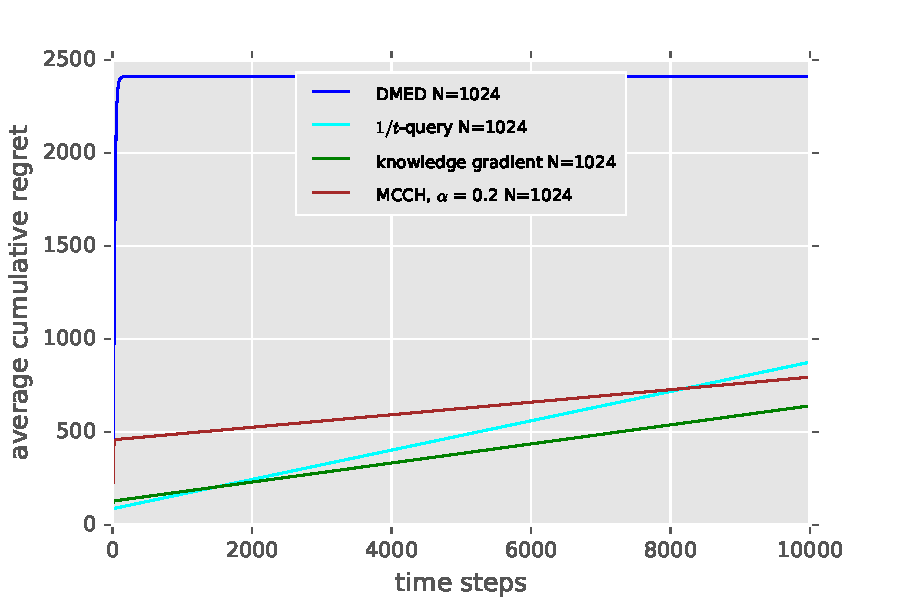
\includegraphics[width=\textwidth]{regret50.pdf}
\caption{Means 0.8 and 0.5, cost $c = 50$.}
\label{fig:regret50}
\end{subfigure}%
~
\begin{subfigure}[b]{0.48\textwidth}
\centering
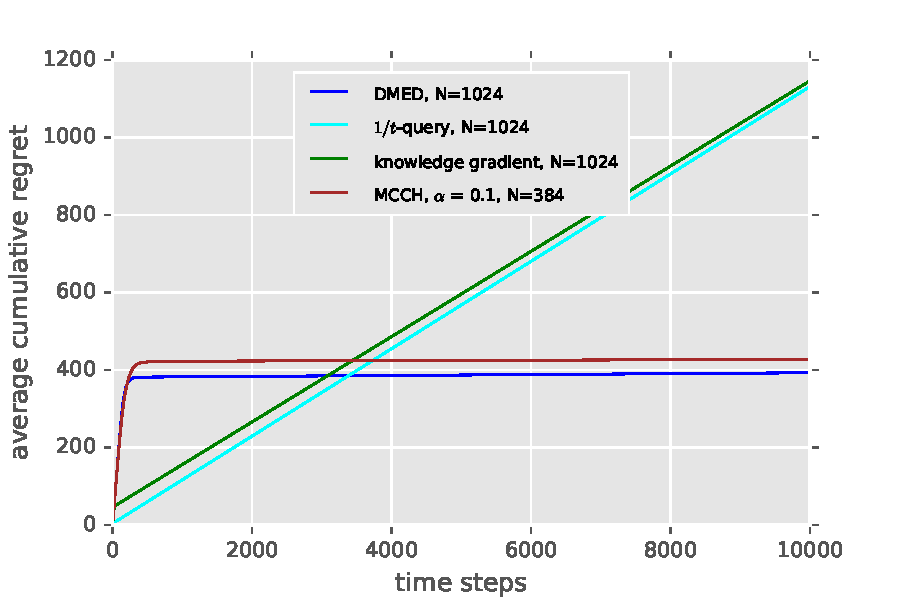
\includegraphics[width=\textwidth]{regret2.pdf}
\caption{Means $0.7, 0.5, 0.4, 0.4, 0.4, 0.4$, cost $c = 2$.}
\label{fig:regret2}
\end{subfigure}
%\end{center}
\caption{
Average cumulative regret for different active bandit algorithms
for Bernoulli arms with horizon $10^4$.
We compare our algorithm \texttt{MCCH} with
knowledge gradient~\citep[Ch.~5]{PowellRyzhov12},
querying with probability $1/t$, and
a \texttt{DMED}~\citep{Honda10} variant that stops querying when
the algorithm selects only one arm.
The latter two algorithms do not take the query cost into account
and this is why they sometimes perform poorly.
}
\label{fig:regret}
\end{figure}

\begin{figure}[t]
%\begin{center}
\centering
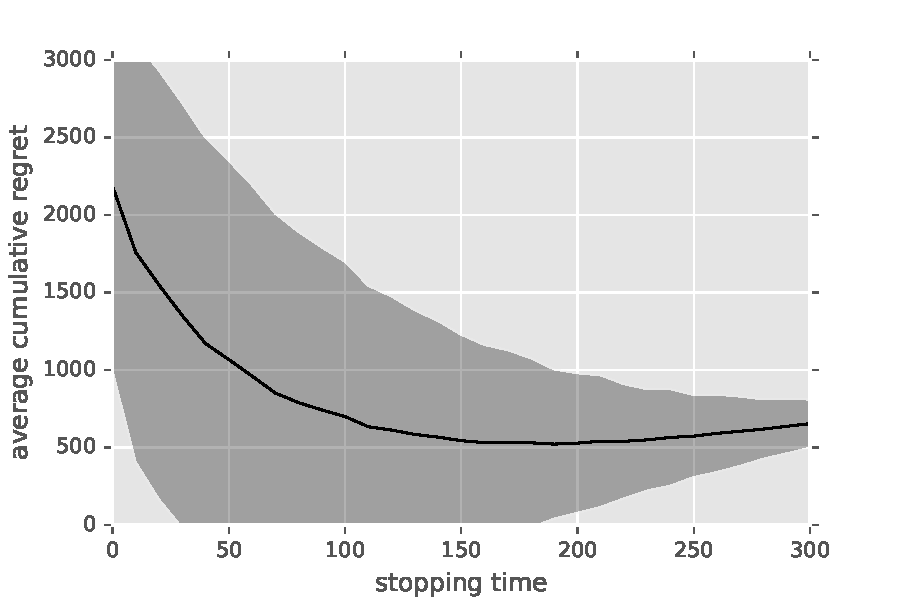
\includegraphics[width=0.48\textwidth]{query-stop.pdf}%
~
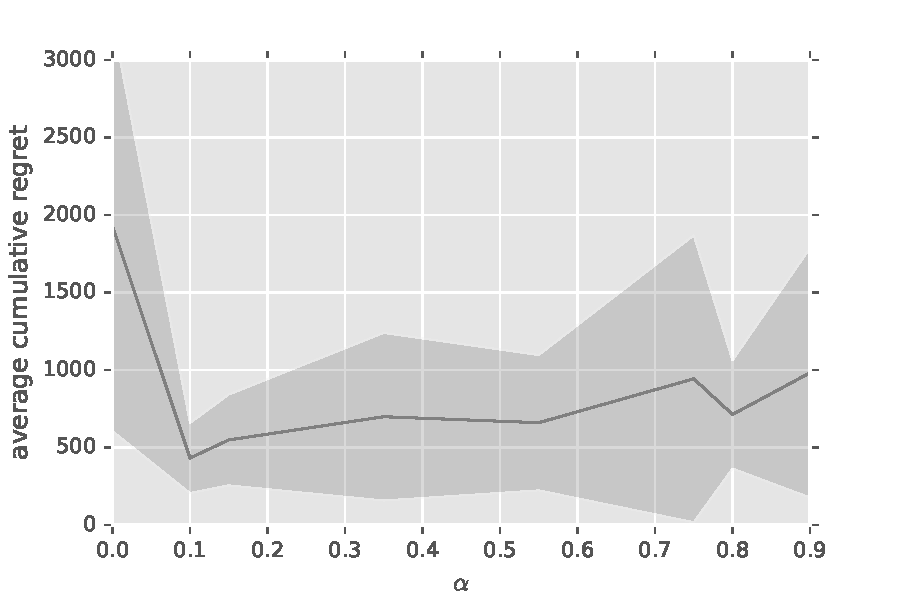
\includegraphics[width=0.48\textwidth]{mcch.pdf}
%\end{center}
\caption{Active 6-armed Bernoulli bandit with means
$0.7, 0.5, 0.4, 0.4, 0.4, 0.4$,
horizon $n = 10^4$, and cost $c = 2$.
We compare two policies:
\texttt{DMED} with a prespecified query stopping time (left)
and \texttt{MCCH}
for different values of the hyperparameter $\alpha$ (right).
The shaded area corresponds to one standard deviation.
\texttt{MCCH} achieves slightly better mean regret,
but also is much more robust to the choice of the hyperparameter.
}
\label{fig:alpha}
\end{figure}


\autoref{fig:regret} shows the average cumulative regret
of different active bandit algorithms for high ($c = 50$) and
moderate ($c = 2$) query costs.
All of these algorithms use \texttt{DMED}~\citep{Honda10}
to select actions.
To be able compute the non-greedy knowledge gradient policy,
we approximate prior, posterior, and likelihood with Gaussian distributions.
While \texttt{MCCH} never quite beats the other algorithms,
it performs more robustly for different query costs.
\autoref{fig:alpha} shows that the choice of its hyperparameter $\alpha$
is not very sensitive,
which makes it better suited than
an optimized fixed (problem-dependent) query stopping time.



%%%%%%%%%%%%%%%%%%%%%%%%%%%%%%%%%%%%%%%%%%%%%%%%%%%%%%%%%%%%%%%
\section{Outlook}
%%%%%%%%%%%%%%%%%%%%%%%%%%%%%%%%%%%%%%%%%%%%%%%%%%%%%%%%%%%%%%%

Open questions/problems:
\begin{itemize}
\item Derive lower bounds on the problem-dependent~\citep[Thm.~2.2]{Bubeck12}
    and cost-dependent regret.
\item Prove (cost-dependent) upper bounds
    on the regret for various algorithms.
\item Is there a performant and efficient parameter-free algorithm?
\end{itemize}


\paragraph{Acknowledgments.}
Tor Lattimore, Reimar Leike, Ryan Lowe, Jessica Taylor, \dots
% The authors would like to acknowledge the use of the University of Oxford Advanced Research Computing (ARC) facility in carrying out this work. \url{http://dx.doi.org/10.5281/zenodo.22558}
% TODO: Following publication please notify ARC by emailing details to 'publications@arc.ox.ac.uk'


%%%%%%%%%%%%%%%%%%%%%%%%%%%%%%%%%%%%%%%%%%%%%%%%%%%%%%%%%%%%%%%
\bibliography{references}


\end{document}
